\chapter{Experimental Apparatus}
\label{CHAPTER:ExperimentalApparatus}

%%%%%%%%%%%%%%%%%%%%%%%%%%%%%%%%%%%%%%%%%%%%%%%%%%%%%%%%%%%%%%%%%%%%%%%%%%%%%%%%%%%%%%%
%%% SECTION
%%%%%%%%%%%%%%%%%%%%%%%%%%%%%%%%%%%%%%%%%%%%%%%%%%%%%%%%%%%%%%%%%%%%%%%%%%%%%%%%%%%%%%%
\section{The Large Hadron Collider}
\label{SECTION:ExperimentalApparatus_LHC}

\colorbox{red}{
\begin{minipage}{0.95\linewidth}
TODO: 

\begin{itemize}
  \item DONE: LHC location, size, particles used, energy usage.
  \item Basics of machine and operation
  \item How instantaneous luminosity is calculated include Instantaneous luminosity equation
  \item Delivered instantaneous luminosity Run I (proton-Proton)
\end{itemize}

\end{minipage}
}

The \gls{LHC}\cite{ARTICLE:LHC Machine} is currently the world's largest particle accelerator and is capable to produce the highest energy particle beam ever made by mankind. This gigantic machine with a total perimeter of 26.7 kilometer was built at \gls{CERN} in a circular tunnel at an average depth of 100 meters below ground under the Franco-Swiss border near Geneva, Switzerland. I Diagram of the LHC tunnel can be found in figure \ref{FIGURE:ExperimentalApparatus_LHCLayoutUnderground}.

\begin{figure}[!htb]
  \centering
  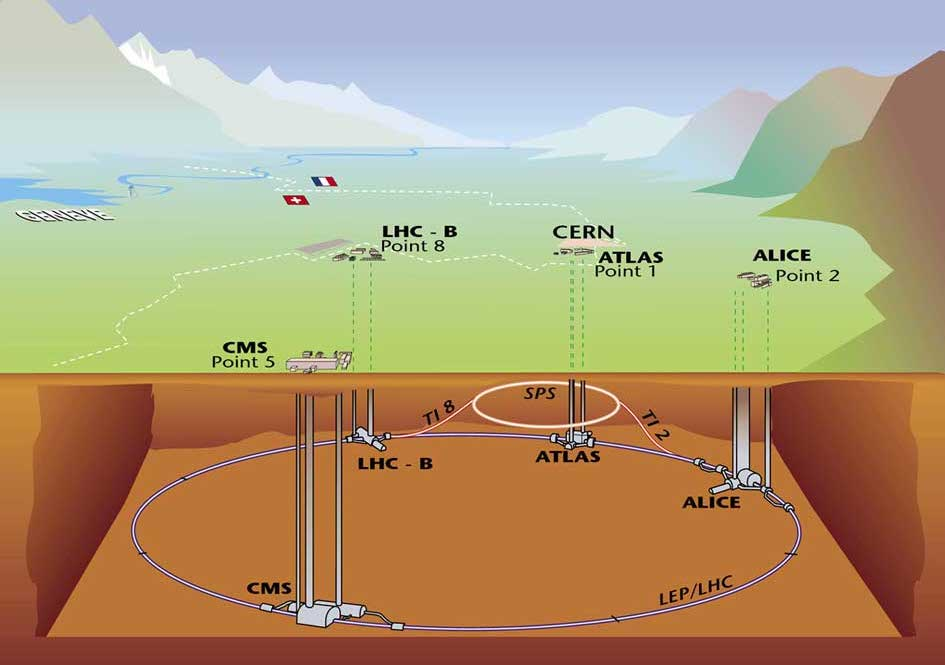
\includegraphics[width=0.50\textwidth]{Chapter02/LHC/Images/LHC_layout_underground.jpg}
  \caption{Underground diagram of the Geneva area showing the \gls{LHC} location.}
  \label{FIGURE:ExperimentalApparatus_LHCLayoutUnderground}
\end{figure}

The \gls{LHC} is a synchrotron machine with the capability to accelerate particles in two separated beam pipes with travel in opposite direction.  These beams only cross and are allowed to collide in four specific points of the accelerator where huge particle detectors are installed to detect the products of such collisions. This experiments are name ATLAS\cite{ARTICLE:TheATLASExperiment}, CMS\cite{ARTICLE:TheCMSExperiment}, LHCb\cite{ARTICLE:TheLHCbExperiment} and ALICE\cite{ARTICLE:TheALICEExperiment}.

The accelerator as its name indicates can collide hadrons, more specifically proton or heavy ions. Up to now 3 modes of operation have been tried according to the particles being collided: proton-proton, proton-lead and lead-lead. Depending on the which configuration is chosen we are basically changing the quantity of nucleons available to each colliding element. The maximum design energy per proton is 7 TeV and for each lead nucleon 2.76 TeV. The design luminosity for proton-proton is of $10^{34}$ $cm^{-2}s^{-1}$ and for lead-lead is of $10^{27}$ $cm^{-2}s^{-1}$.

The \gls{LHC} is only the last element of a complex accelerator chain which step by step increases the energy of the particles. Protons are initially obtained by stipping the electrons of hydrogen gas. The are then accelerated at the \gls{LINAC2} up to the energy of 50 MeV. After this initial step they are injected into the \gls{PSB} and the energy ramps ups to 1.4 GeV. After protons are passed to the \gls{PS} where energy futher increases to 25 GeV subsequently they are the injected into the \gls{SPS} where the particle energy level reached 450 GeV. Finally, protons pass to the \gls{LHC} where they can be accelerated to a maximum energy of 7 TeV. A simplified diagram of the \gls{CERN} accelerator chain can be found in figure \ref{FIGURE:ExperimentalApparatus_LHCAccelaratorChain}.

\begin{figure}[!htb]
  \centering
  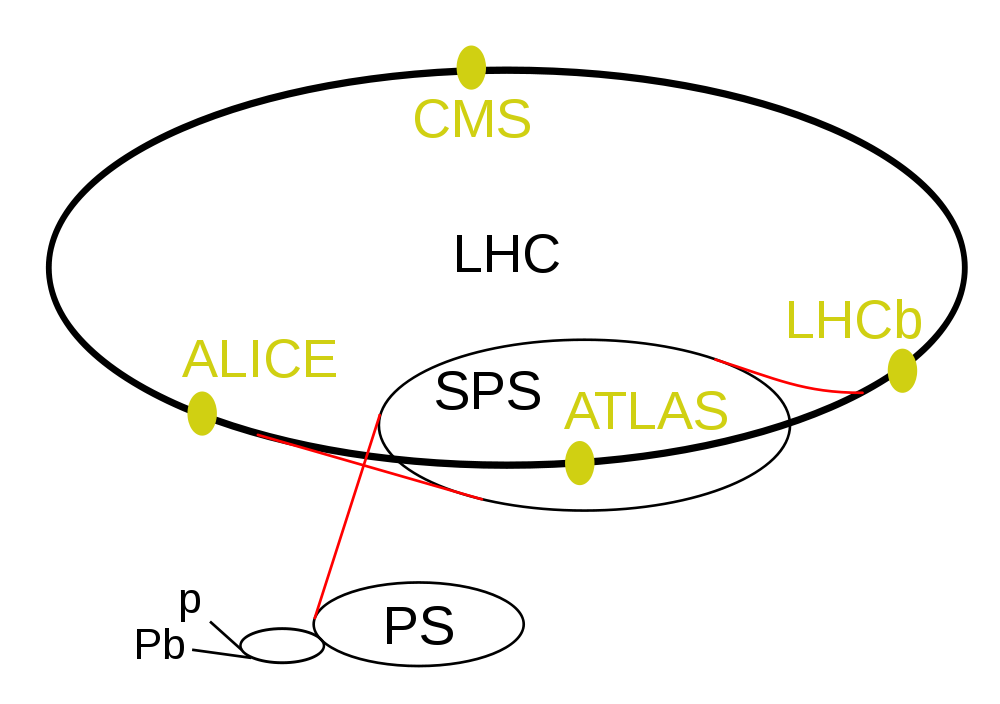
\includegraphics[width=0.50\textwidth]{Chapter02/LHC/Images/LHCAccelaratorChain.png}
  \caption{CERN Large Hadron Collider Experiment accelerator diagram.}
  \label{FIGURE:ExperimentalApparatus_LHCAccelaratorChain}
\end{figure}

Normal operation of the \gls{LHC} therefore depends on the the upstream accelerators availability. The typically turn around time, the time necessary to stop the accelerator from running and restart collisions is around 2 hours. When stable beams are achieved, a single proton fill can be used to collide protons up to 24 hours, but it is common to restart more frequently to take profit of the higher collision rates possible right at the beginning of a new fill.

Some of the key parameters of the LHC proton-proton and lead-lead operation can be found in table \ref{TABLE:ExperimentalApparatus_LHCMachineParameters}.

\begin{table}[!htb]
  \centering
  \begin{threeparttable}
    \begin{tabular}{|lcccc|}
    \hline 
                                  &              &           \textit{pp} &         \textbf{HI} &  \\
    \hline\hline
    Energy per nucleon            & E            &                     7 &                2.76 &                 $\TeV$ \\
    Dipole field at 7 TeV         & \textit{B}   &                  8.33 &                8.33 &               $\tesla$ \\
    Design Luminosity\tnote{*}    & $\mathcal{L}$ &            $10^{34}$ &           $10^{27}$ & $\cm^{-2}\second^{-1}$ \\
    Bunch separation              &              &                    25 &                 100 &                  $\ns$ \\
    No. of bunches                & $k_B$        &                  2808 &                 592 &                        \\
    No. particles per bunch       & $N_p$        & $1.15 \times 10^{11}$ & $7.0 \times 10^{7}$ &                        \\
    \hline
    \hline
    \textbf{Collisions}           &              &  &  &  \\
    \hline
    $\beta$-value at IP           & $\beta^{*}$  &                  0.55 &                 0.5 &        $\meter$ \\
    RMS beam radius at IP         & $\sigma^{*}$ &                  16.7 &                15.9 &  $\micro\meter$ \\
    Luminosity lifetime           & $\tau_L$     &                    15 &                   6 &         $\hour$ \\
    Number of collisions/crossing & $n_c$        &          $\approx 20$ &                   - &                 \\
    \hline
    \end{tabular}
    \begin{tablenotes}
      \item[*] For heavy-ion (HI) operation the design luminosity for Pb-Pb collisions is given.
    \end{tablenotes}
  \end{threeparttable}
  \caption[LHC parameters relevant for detectors]{The machine parameters relevant for the 
                                                  LHC detectors.\cite{CMSTDR:CMSPhysicsVol1}}
  \label{TABLE:ExperimentalApparatus_LHCMachineParameters}
\end{table}


\begin{figure}[!htb]
  \centering
  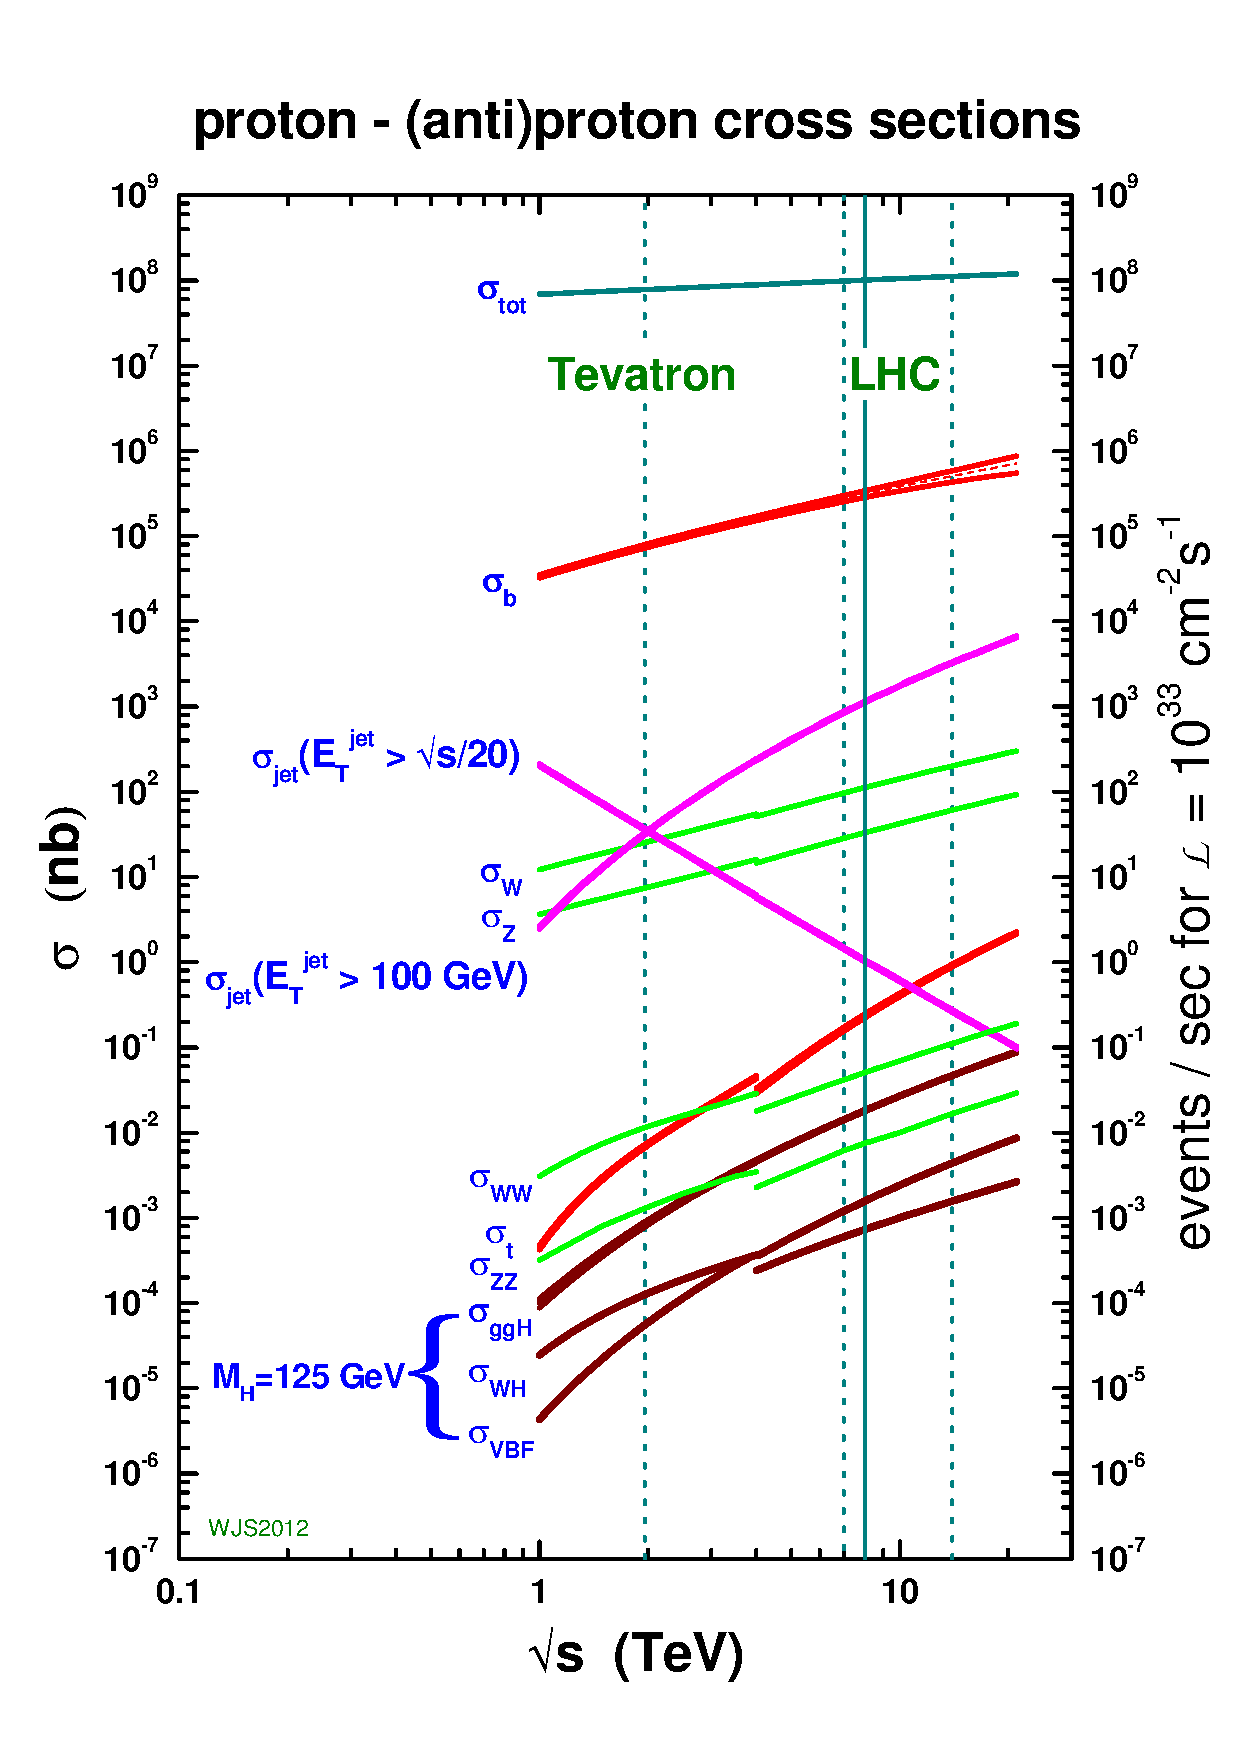
\includegraphics[width=0.50\textwidth]{Chapter02/LHC/Images/crosssections2012_v5}
  \caption{Cross sections for several processes for collisions of antiproton-proton and proton-proton as a function of the center of mass energy\cite{ARTICLE:TheCMSExperiment}.}
  \label{FIGURE:ExperimentalApparatus_LHCCrossSections}
\end{figure}

At the \gls{LHC} we are looking for extremely rare processes as is can be seen in figure \ref{FIGURE:ExperimentalApparatus_LHCCrossSections} the production cross section of a \gls{SM} Higgs boson is more than 9 orders of magnitude smaller than the total proton-proton cross section. 

To be able to record and study such rare processes we need to produce a significant amount of collisions. For this purpose the LHC was designed to operate at high instantaneous luminosity, L. This quantity is defined as,

\begin{equation}
L=\frac{N_{b}^{2}n_{b}f_{\text{rev}}\gamma}{4\pi\epsilon_{n}\beta^{*}}F,
\end{equation}

where $N_{b}$ is the number of protons per bunch, $n_{b}$ is the number of bunches, $f_{\text{rev}}$ is the frequency of revolution, $\gamma$ is the Lorentz factor, $\epsilon_{n}$ is the normalized emittance, $f_{\text{rev}}$ is the beta function at the collision point and $F$ is the reduction factor due to the crossing angle.

%%%%%%%%%%%%%%%%%%%%%%%%%%%%%%%%%%%%%%%%%%%%%%%%%%%%%%%%%%%%%%%%%%%%%%%%%%%%%%%%%%%%%%%
%%% SUBSECTION
%%%%%%%%%%%%%%%%%%%%%%%%%%%%%%%%%%%%%%%%%%%%%%%%%%%%%%%%%%%%%%%%%%%%%%%%%%%%%%%%%%%%%%%
\subsection{Delivered Luminosity}

\begin{figure}[!htb]
  \centering
  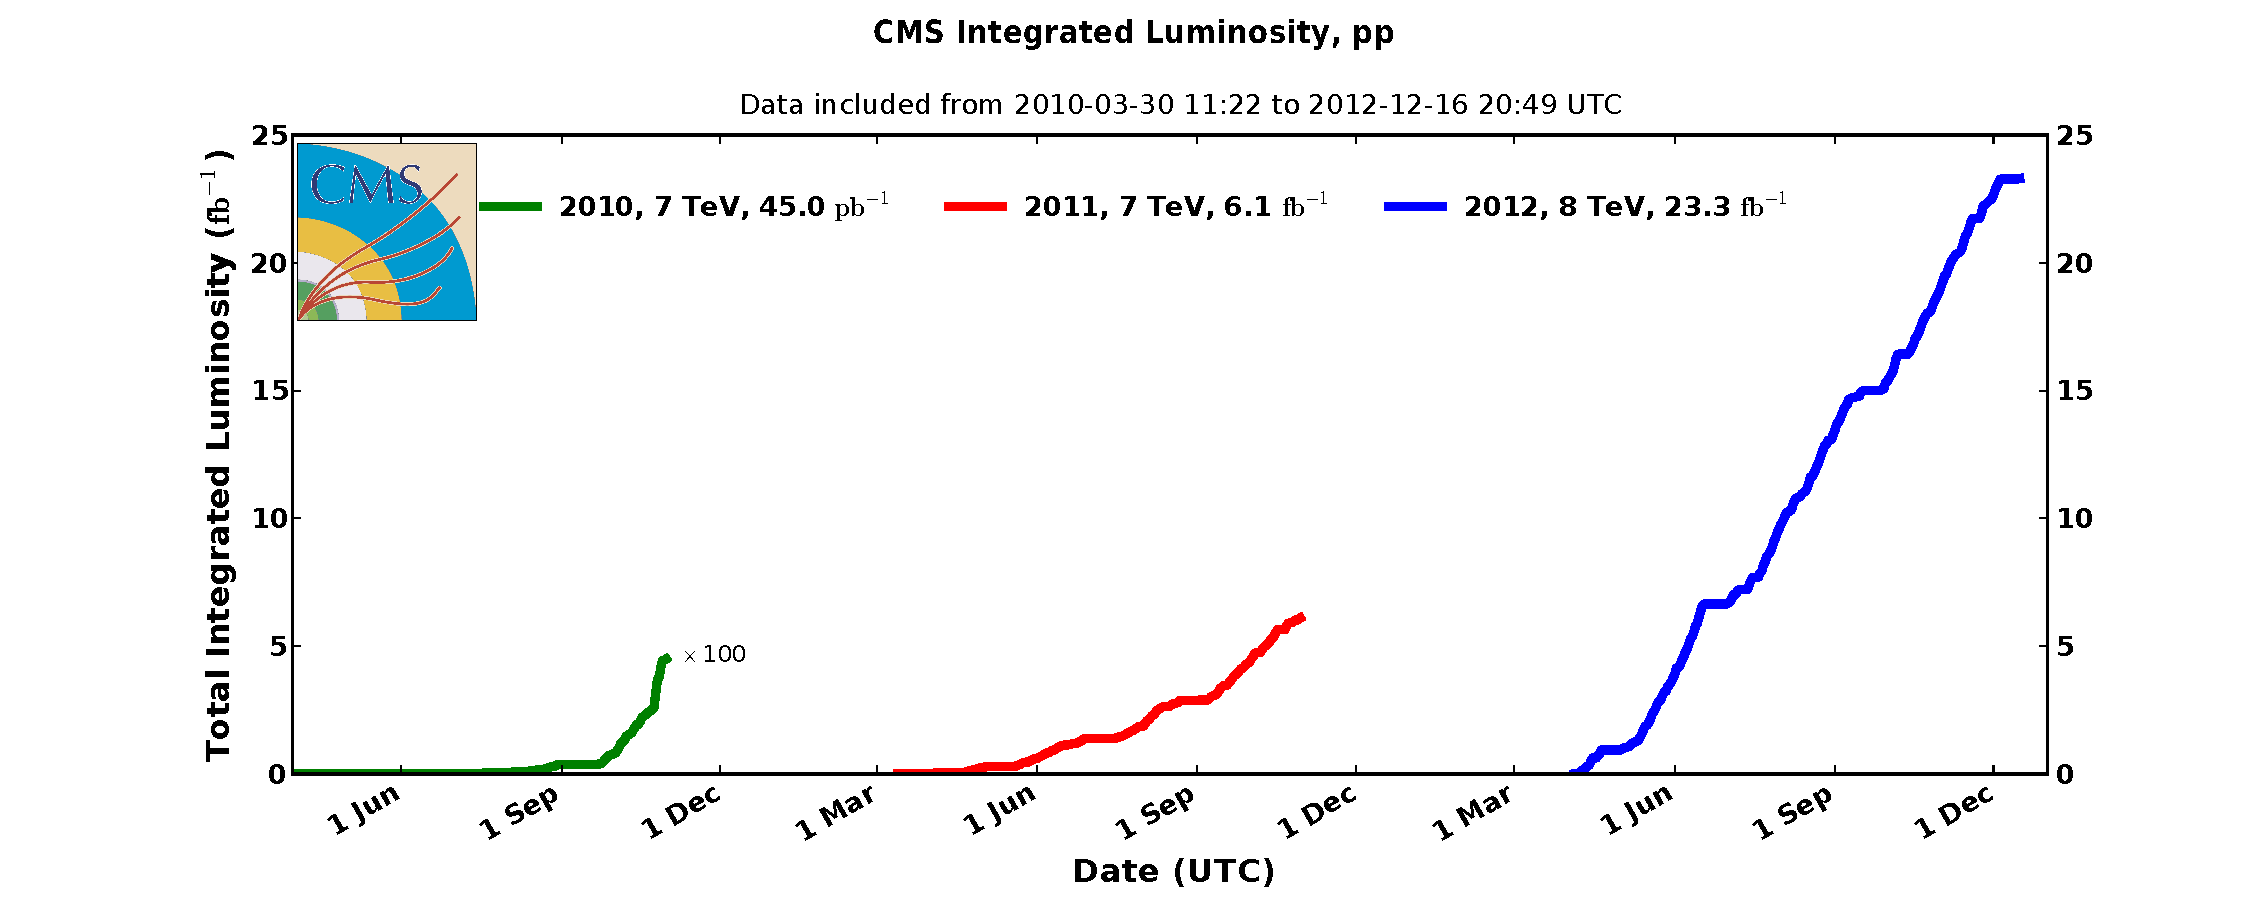
\includegraphics[width=1.00\textwidth]{Chapter02/CMS/Images/CMS_IntegratedLumi_pp_2010-2012}
  \caption{Cumulative luminosity versus day delivered to CMS during stable beams and for p-p collisions. This is shown for 2010 (green), 2011 (red) and 2012 (blue) data-taking.}
  \label{FIGURE:ExperimentalApparatus_CMS_IntegratedLumi_pp_2010-2012}
\end{figure}

\begin{figure}[!htb]
  \centering
  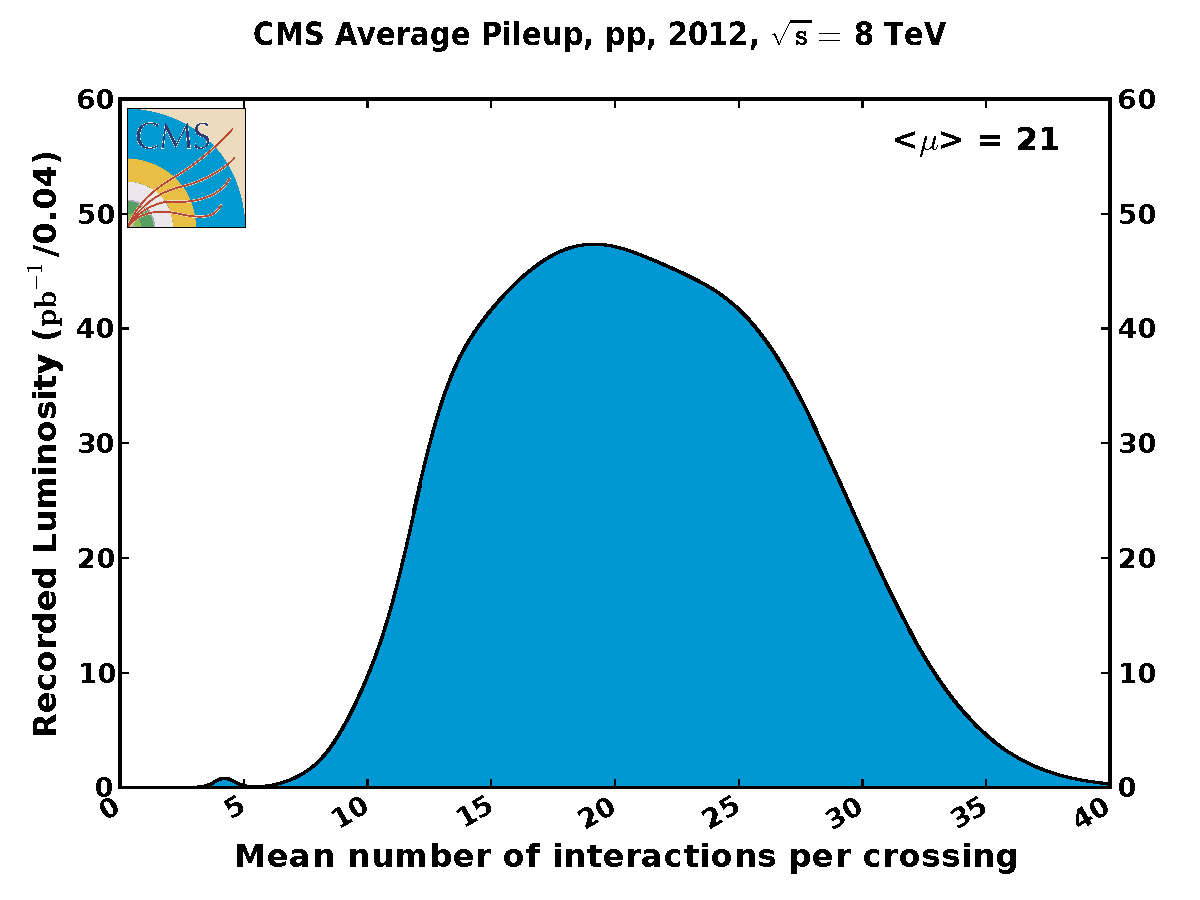
\includegraphics[width=0.50\textwidth]{Chapter02/CMS/Images/CMS_PileIp_pp_2012}
  \caption{Mean number of interactions per bunch crossing at the CMS experiment during 2012.}
  \label{FIGURE:ExperimentalApparatus_CMS_PileIp_pp_2012}
\end{figure}

\section{The Compact Muon Solenoid Experiment}
\label{SECTION:ExperimentalApparatus_CMS}

The \gls{CMS} experiment is a general purpose experiment located at point 5 of the \gls{LHC}. It was designed to study collisions at its centre and is composed os several sub-systems in an classic onion shaped structure.


%%%%%%%%%%%%%%%%%%%%%%%%%%%%%%%%%%%%%%%%%%%%%%%%%%%%%%%%%%%%%%%%%%%%%%%%%%%%%%%%%%%%%%%
%%% SUBSECTION
%%%%%%%%%%%%%%%%%%%%%%%%%%%%%%%%%%%%%%%%%%%%%%%%%%%%%%%%%%%%%%%%%%%%%%%%%%%%%%%%%%%%
\subsection{Geometry and conventions}


%%%%%%%%%%%%%%%%%%%%%%%%%%%%%%%%%%%%%%%%%%%%%%%%%%%%%%%%%%%%%%%%%%%%%%%%%%%%%%%%%%%%%%%
%%% SUBSECTION
%%%%%%%%%%%%%%%%%%%%%%%%%%%%%%%%%%%%%%%%%%%%%%%%%%%%%%%%%%%%%%%%%%%%%%%%%%%%%%%%%%%%
\subsection{Inner tracking system}
\label{SUBSECTION:ExperimentalApparatus_CMS_Tracker}

% Writing points:
% * Closest detector to beam, measures trajectories of charged particles
% * With magnetic field measures momentum and charge of this particles
% * Allows vertexing (primary and secundary)
% * Different regions different occupancy
% * Final arranagement

The inner tracking system is the closest detector to the beam axis and the interaction region. Its function is to measure the trajectory of all charged particles, like electrons, charged hadrons and muons with momentum above 1 $GeV$ being produced at each \gls{LHC} collision. With the help of the strong magnetic field produced by the \gls{CMS} magnet particle trajectory is bent allowing for charge and momentum determination. With the resulting tracks is it then possible to determine the primary vertex of interaction as well as vertexes of other interactions or even displaced vertexes from the decay of long lived particles like B mesons. 

Building a tracking system for a \gls{LHC} experiment is very challenging. At design luminosity an average of 1000 particles will hit such system at a rate approaching 40 $MHz$ , leading to high hit density and high rate. It is therefore desirable to have a fast, efficient and high granularity system where at each layer the occupancy should be at or below $1\%$. On the other hand each layer should be as thin as possible in order to not change the incoming particles trajectory or make them lose too much energy. The detector should also be radiation hard and survive for a period of at least 10 years due to its importance and location. This design requirements lead to a tracker design entirely based on silicon detector technology. 

The volume near the interaction point can be split according to the charged particle flux into three regions depending on the charged particle flux.

\begin{itemize}
  \item $r<10$ $cm$: highest particle flux, up to $\approx 10^8 $ $cm^{-2}s^{-1}$ at $r \approx 4$ $cm$, pixel detectors are used. The pixel size is $\approx 100 \times 150$ $\mu m^2$, which translates into an occupancy of $10^{-4}$ per \gls{LHC} bunch crossing.
  \item $20<r<55$ $cm$: particle flux decreases enough to use silicon micro-strips with a minimum cell size of 10 cm $\times$ 80 $\mu m$, leading to an occupancy of $\approx 2-3\%$ per \gls{LHC} bunch crossing.
  \item $50<r<110$ $cm$: most outer region of the tracker, particle flux is low enough the larger pitch silicon micro-strips can be used. The maximum cell size is of 25 $cm$ $\times$ 180 $\mu m$, occupancy is of the order of $\approx 1\%$.
\end{itemize}

The \gls{CMS} tracker final configuration is composed of a pixel detector with three barrel layers at radii between 4.4 $cm$ and 10.2 $cm$ and 2 disks on each side of the barrel. And a silicon strip tracker with 10 barrel detection layers extending up to 1.1 $m$ with 3 plus 9 disks on each side of the barrel. A schematic of the detector module distribution can be found in figure \ref{FIGURE:ExperimentalApparatus_CMS_Tracker_Layout}. This detector has an acceptance covering up to pseudorapidity of $|\eta|<2.5$ and has a total active area of about 200 $m^2$ making the largest silicon tracker ever built. 

\begin{figure}[!htb]
  \centering
  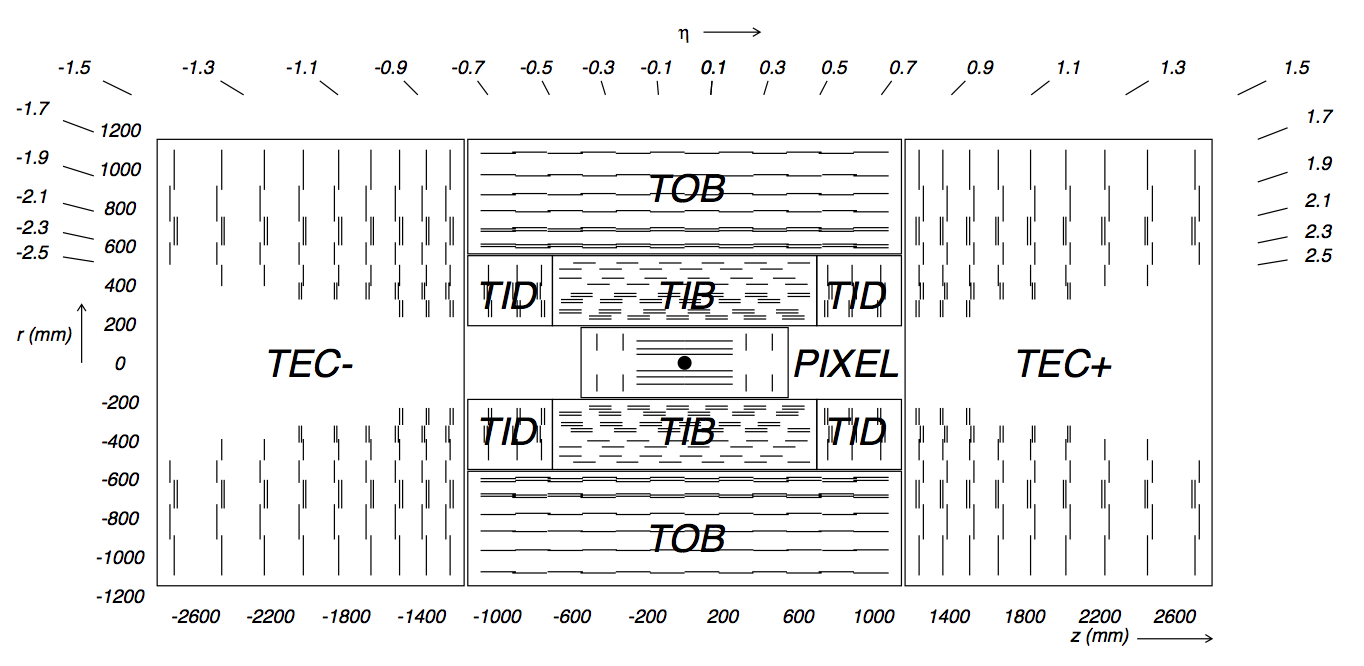
\includegraphics[width=1.0\textwidth]{Chapter02/CMS/Images/CMS_Tracker_Layout.png}
  \caption{Schematic cross section of the CMS tracker. Each line represent a detector module. Double lines represent dual surface back-to-back detector modules.}
  \label{FIGURE:ExperimentalApparatus_CMS_Tracker_Layout}
\end{figure}

%%%%%%%%%%%%%%%%%%%%%%%%%%%%%%%%%%%%%%%%%%%%%%%%%%%%%%%%%%%%%%%%%%%%%%%%%%%%%%%%%%%%%%%
%%% SUBSECTION
%%%%%%%%%%%%%%%%%%%%%%%%%%%%%%%%%%%%%%%%%%%%%%%%%%%%%%%%%%%%%%%%%%%%%%%%%%%%%%%%%%%%
\subsection{Electromagnetic Calorimeter}
\label{SUBSECTION:ExperimentalApparatus_CMS_ECAL}
% STATUS: DONE (just with MSc input, and needs review)

The \gls{ECAL} is an hermetic energy measurement system comprised of 61200 lead tungstate ($PbWO_4$) crystals mounted in the barrel and 7324 crystals in each of the 2 endcaps.

Lead tungstate had a fairly high density (8.28 $g/cm^3$), has a short radiation length (0.89 $cm$) and a small Moliere redius (2.2 $cm$). The crystals also have a fast scintillation decay time emitting 80\% of the light yield in 25 $ns$ (the minimal bunch crossing time at the LHC). This characteristics make it a good choice for an electromagnetic calorimeter allowing a compact design with fine granularity. However, this crystals emit a fairly low light yield (30 $\gamma/MeV$) which requires the use of photo-detectors with intrinsic gain which will preform well inside a magnitic field. In the barrel region silicon \gls{APD} are used and \gls{VPT} are used in the endcaps. To guarantee good response from both crystals and \gls{APD} it is necessary to have system thermal stability, with the goal being temperature variation of less than 0.1º C.

The barrel section, the \gls{EB}, has an inner radius of 129 $cm$ and is composed of 36 identical ``supermodules``, each covers the barrel length and corresponding to a pseudo-rapidity interval of $0<|\eta|<1.479$. The crystals are quasi-projective (the axes are tilted at 3º with respect to the line from the nominal vertex position) and cover 0.0174 (i.e. 1º ) in $\Delta\phi$ and $\Delta\eta$. The crystals have a front face cross-section of $\approx 22\times22$ $mm^2$ and a length of 230 $mm$, corresponding to 25.8 $X_0$.

The endcap section, the \gls{EE}, is at a distance of 314 cm from the vertex and covering a pseudorapidity range of $1.479<|\eta|<3.0$, are each structured as 2 “Dees”, consisting of semi-circular aluminium plates from which are cantilevered structural units of $5\times5$ crystals, known as “supercrystals”.

%%%%%%%%%%%%%%%%%%%%%%%%%%%%%%%%%%%%%%%%%%%%%%%%%%%%%%%%%%%%%%%%%%%%%%%%%%%%%%%%%%%%%%%
%%% SUBSECTION
%%%%%%%%%%%%%%%%%%%%%%%%%%%%%%%%%%%%%%%%%%%%%%%%%%%%%%%%%%%%%%%%%%%%%%%%%%%%%%%%%%%%
\subsection{Hadronic Calorimeter}
\label{SUBSECTION:ExperimentalApparatus_CMS_HCAL}

The \gls{HCAL}

%%%%%%%%%%%%%%%%%%%%%%%%%%%%%%%%%%%%%%%%%%%%%%%%%%%%%%%%%%%%%%%%%%%%%%%%%%%%%%%%%%%%%%%
%%% SUBSECTION
%%%%%%%%%%%%%%%%%%%%%%%%%%%%%%%%%%%%%%%%%%%%%%%%%%%%%%%%%%%%%%%%%%%%%%%%%%%%%%%%%%%%
\subsection{Solenoid Magnet}
\label{SUBSECTION:ExperimentalApparatus_CMS_Magnet}

\begin{table}[!htb]
  \centering
  \begin{tabular}{|l|c|}
  \hline
  Parameter & Value \\
  \hline\hline
  Field           & 4 T \\
  Inner Bore      & 5.9 m \\
  Length          & 12.9 m \\
  Number of turns & 2168 \\
  Current         & 19.5 kA \\
  Stored Energy   & 2.7 GJ \\
  Hoop Stress     & 64 atm \\
  \hline
  \end{tabular}
  \caption[Parameters of the CMS superconducting solenoid]{Parameters of the CMS superconducting solenoid}
  \label{TABLE:ExperimentalApparatus_CMSMagnetParameters}
\end{table}


%%%%%%%%%%%%%%%%%%%%%%%%%%%%%%%%%%%%%%%%%%%%%%%%%%%%%%%%%%%%%%%%%%%%%%%%%%%%%%%%%%%%%%%
%%% SUBSECTION
%%%%%%%%%%%%%%%%%%%%%%%%%%%%%%%%%%%%%%%%%%%%%%%%%%%%%%%%%%%%%%%%%%%%%%%%%%%%%%%%%%%%
\subsection{Muon System}
\label{SUBSECTION:ExperimentalApparatus_CMS_Mouns}

%%%%%%%%%%%%%%%%%%%%%%%%%%%%%%%%%%%%%%%%%%%%%%%%%%%%%%%%%%%%%%%%%%%%%%%%%%%%%%%%%%%%%%%
%%% SUBSECTION
%%%%%%%%%%%%%%%%%%%%%%%%%%%%%%%%%%%%%%%%%%%%%%%%%%%%%%%%%%%%%%%%%%%%%%%%%%%%%%%%%%%%
\subsection{Data Acquisition System}
\label{SUBSECTION:ExperimentalApparatus_CMS_DAQ}

The \gls{DAQ}

%%%%%%%%%%%%%%%%%%%%%%%%%%%%%%%%%%%%%%%%%%%%%%%%%%%%%%%%%%%%%%%%%%%%%%%%%%%%%%%%%%%%%%%
%%% SUBSECTION
%%%%%%%%%%%%%%%%%%%%%%%%%%%%%%%%%%%%%%%%%%%%%%%%%%%%%%%%%%%%%%%%%%%%%%%%%%%%%%%%%%%%
\subsection{Trigger System}
\label{SUBSECTION:ExperimentalApparatus_CMS_Trigger}

The \gls{L1T} and \gls{HLT}

%%%%%%%%%%%%%%%%%%%%%%%%%%%%%%%%%%%%%%%%%%%%%%%%%%%%%%%%%%%%%%%%%%%%%%%%%%%%%%%%%%%%%%%
%%% SUBSECTION
%%%%%%%%%%%%%%%%%%%%%%%%%%%%%%%%%%%%%%%%%%%%%%%%%%%%%%%%%%%%%%%%%%%%%%%%%%%%%%%%%%%%
\subsection{Computing}
\label{SUBSECTION:ExperimentalApparatus_CMS_Computing}

The \gls{DQM} 

%%%%%%%%%%%%%%%%%%%%%%%%%%%%%%%%%%%%%%%%%%%%%%%%%%%%%%%%%%%%%%%%%%%%%%%%%%%%%%%%%%%%%%%
%%% SUBSECTION
%%%%%%%%%%%%%%%%%%%%%%%%%%%%%%%%%%%%%%%%%%%%%%%%%%%%%%%%%%%%%%%%%%%%%%%%%%%%%%%%%%%%
\subsection{Run II Updgrades}
\label{SUBSECTION:ExperimentalApparatus_CMS_RUNII}

The upgrade tdr \cite{CMSTDR:CMSL1Upgrade}.
